\documentclass[border=10pt]{standalone}
\usepackage{tikz}
\usetikzlibrary{arrows.meta, positioning, calc, fit, backgrounds}
\usepackage{amsmath}

\definecolor{frozen}{RGB}{180,210,240}
\definecolor{newmod}{RGB}{255,220,130}
\definecolor{ditbg}{RGB}{230,235,250}
\definecolor{xattnbg}{RGB}{195,240,195}
\definecolor{lossbg}{RGB}{195,235,195}

\tikzset{
  B/.style={draw, rounded corners=3pt, minimum height=0.7cm, align=center, font=\small, thick},
  F/.style={B, fill=frozen},
  N/.style={B, fill=newmod},
  W/.style={B, fill=white},
  G/.style={B, fill=lossbg},
  X/.style={B, fill=xattnbg},
  a/.style={-{Stealth[length=2.5mm]}, thick},
  d/.style={-{Stealth[length=2.5mm]}, thick, dashed, red!60!black},
  t/.style={font=\scriptsize\ttfamily, text=blue!70!black},
  lb/.style={font=\scriptsize},
}

\begin{document}
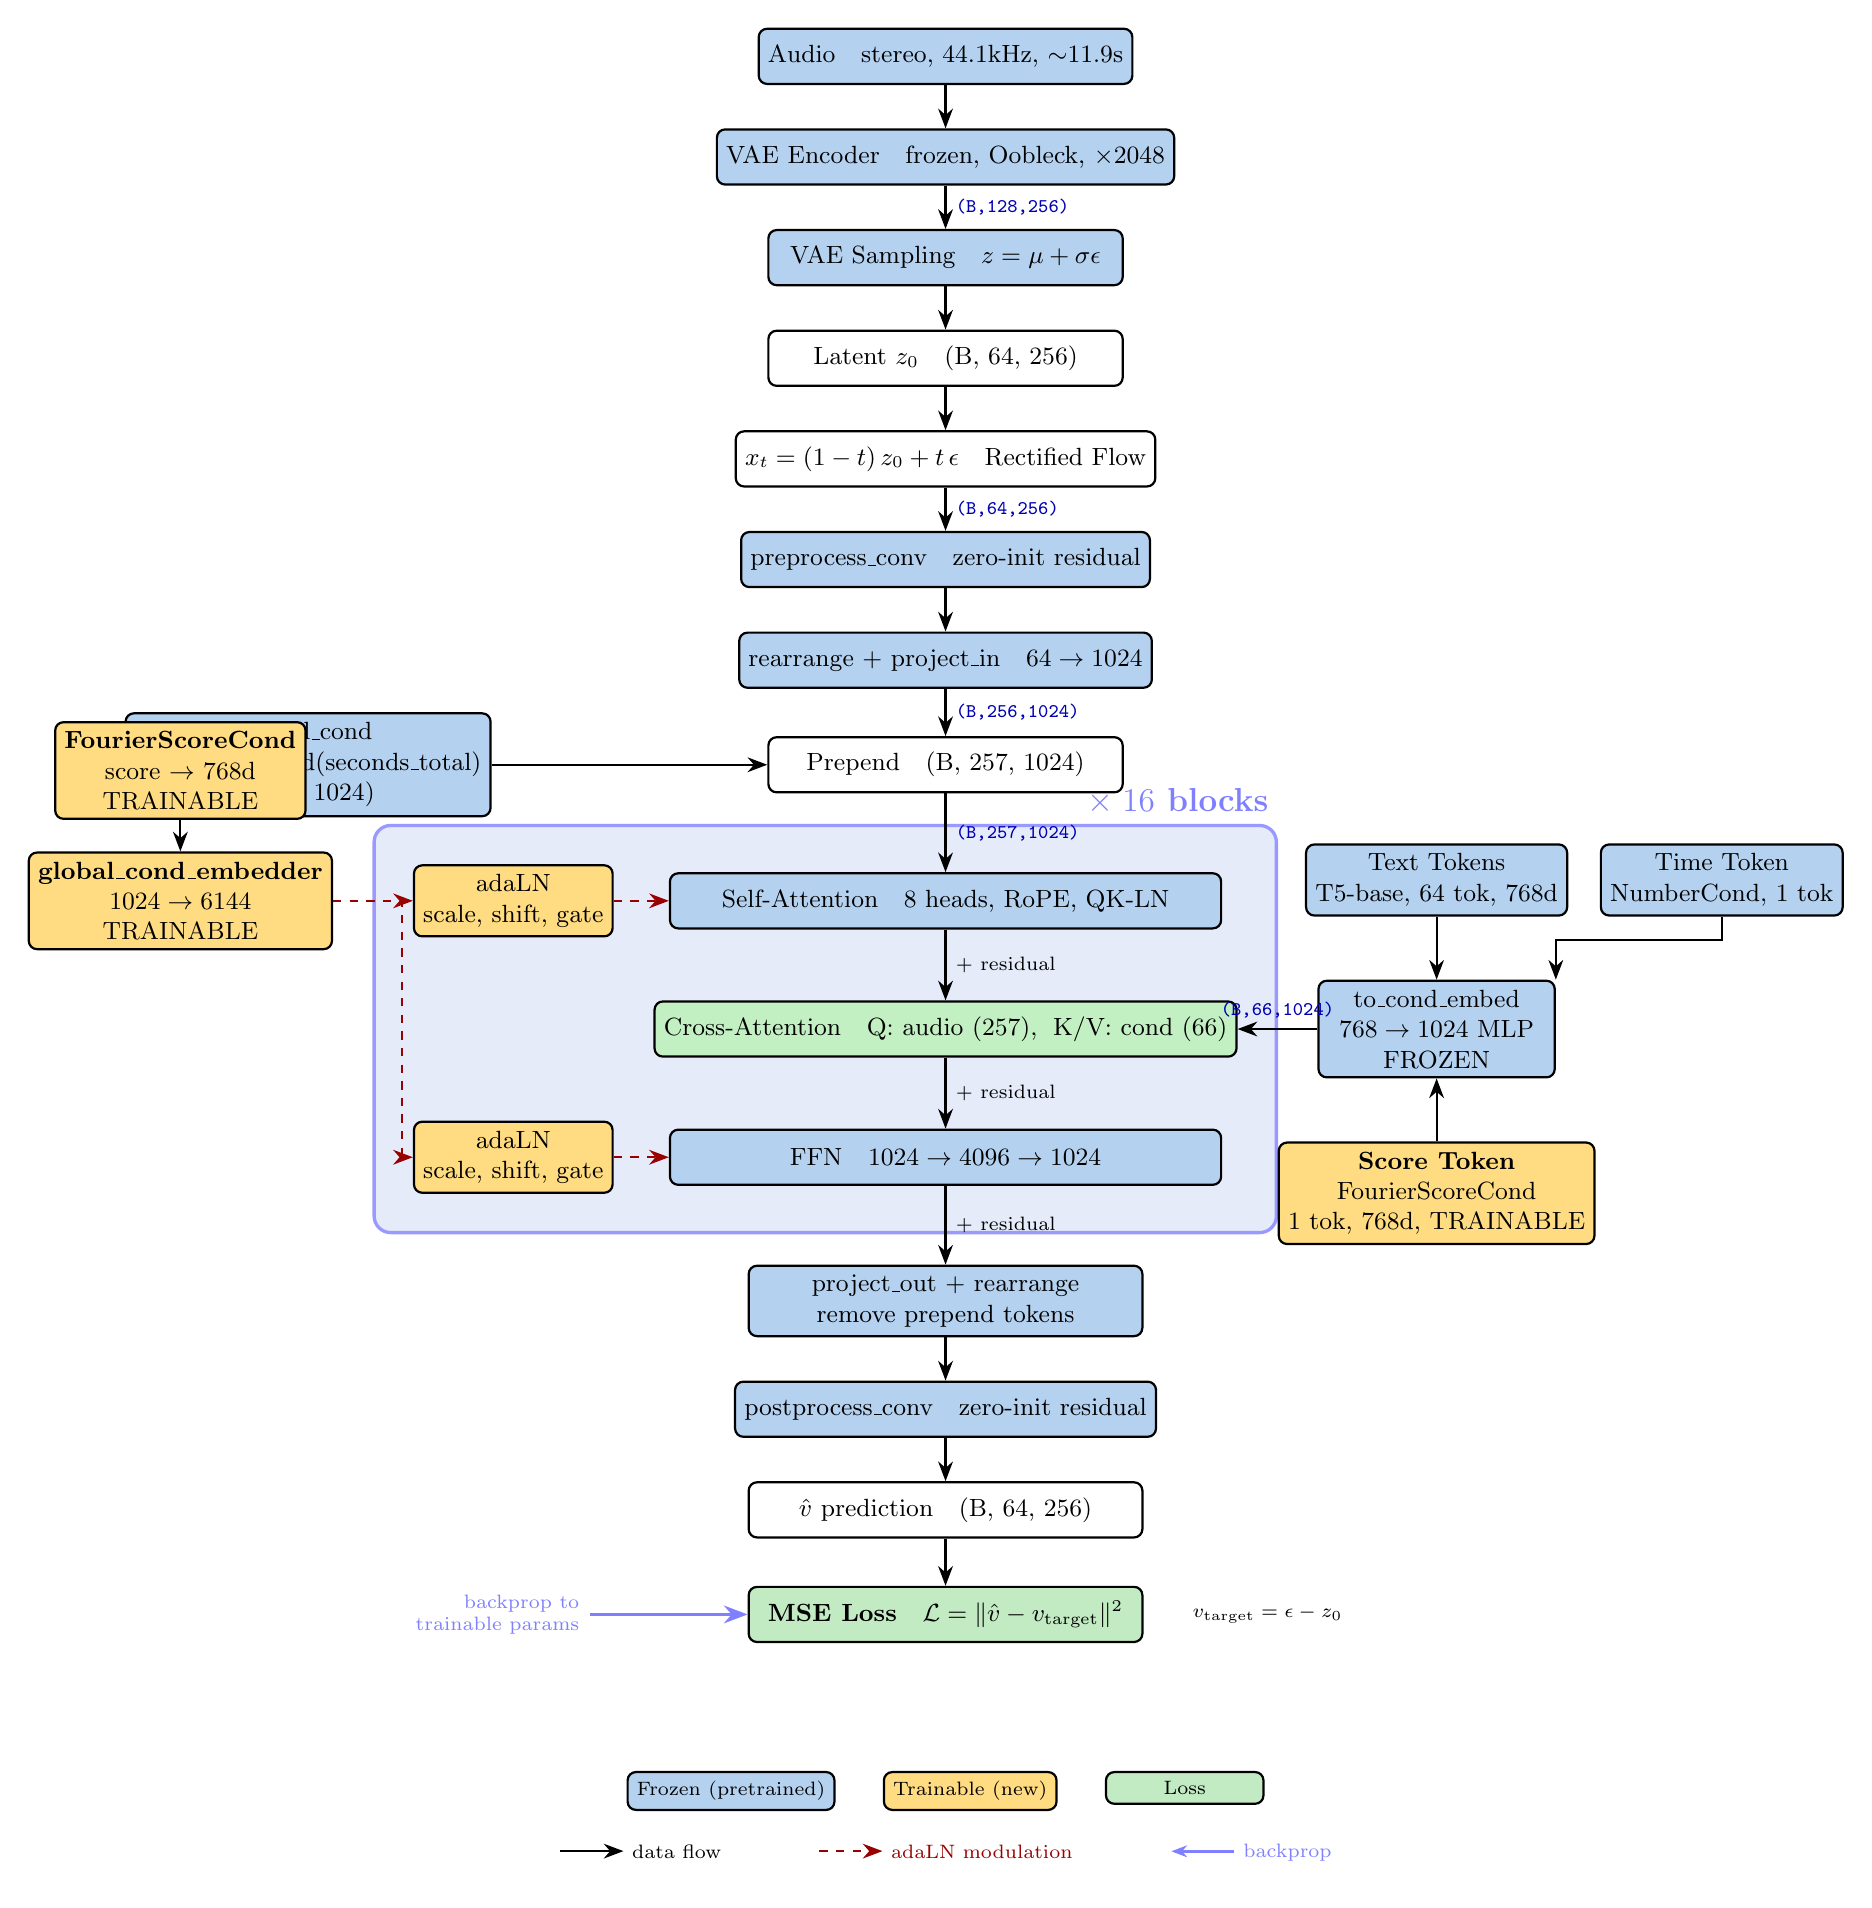
\begin{tikzpicture}[node distance=0.55cm]

% ==================== TOP: Audio → Latent ====================
\node[F, minimum width=4.5cm] (audio) {Audio\quad\lb{stereo, 44.1kHz, $\sim$11.9s}};
\node[F, minimum width=4.5cm, below=of audio] (vae) {VAE Encoder\quad\lb{frozen, Oobleck, $\times$2048}};
\node[F, minimum width=4.5cm, below=of vae] (samp) {VAE Sampling\quad\lb{$z=\mu+\sigma\epsilon$}};
\node[W, minimum width=4.5cm, below=of samp] (z0) {Latent $z_0$\quad\lb{(B, 64, 256)}};
\node[W, minimum width=4.5cm, below=of z0] (xt) {$x_t = (1-t)\,z_0 + t\,\epsilon$\quad\lb{Rectified Flow}};
\node[F, minimum width=4.5cm, below=of xt] (preconv) {preprocess\_conv\quad\lb{zero-init residual}};
\node[F, minimum width=4.5cm, below=of preconv] (projin) {rearrange + project\_in\quad\lb{$64 \to 1024$}};

\draw[a](audio)--(vae);
\draw[a](vae)--node[right,t]{(B,128,256)}(samp);
\draw[a](samp)--(z0);
\draw[a](z0)--(xt);
\draw[a](xt)--node[right,t]{(B,64,256)}(preconv);
\draw[a](preconv)--(projin);

% ==================== PREPEND ====================
\node[W, minimum width=4.5cm, below=0.6cm of projin] (prepend) {Prepend\quad\lb{(B, 257, 1024)}};
\draw[a](projin)--node[right,t]{(B,256,1024)}(prepend);

% global_cond — seconds_total (left of prepend, clean)
\node[F, left=3.5cm of prepend, minimum width=3cm] (gcond) {global\_cond\\\lb{to\_global\_embed(seconds\_total)}\\\lb{(B, 1, 1024)}};
\draw[a](gcond)--(prepend);

% ==================== DiT BLOCK x16 ====================

% Main blocks — wide enough for labels
\node[F, below=1cm of prepend, minimum width=7cm] (sa) {Self-Attention\quad\lb{8 heads, RoPE, QK-LN}};
\node[X, below=0.9cm of sa, minimum width=7cm] (xa) {Cross-Attention\quad\lb{Q: audio (257),\; K/V: cond (66)}};
\node[F, below=0.9cm of xa, minimum width=7cm] (ffn) {FFN\quad\lb{$1024 \to 4096 \to 1024$}};

\draw[a](prepend)--node[right,t]{(B,257,1024)}(sa);
\draw[a](sa)--node[right,lb]{+ residual}(xa);
\draw[a](xa)--node[right,lb]{+ residual}(ffn);

% ---- adaLN (inside box, left) ----
\node[N, left=0.7cm of sa, minimum width=2cm, yshift=0cm] (aln1) {adaLN\\\lb{scale, shift, gate}};
\node[N, left=0.7cm of ffn, minimum width=2cm, yshift=0cm] (aln2) {adaLN\\\lb{scale, shift, gate}};
\draw[d](aln1.east)--(sa.west);
\draw[d](aln2.east)--(ffn.west);

% ---- x16 bounding box ----
\begin{scope}[on background layer]
  \node[draw=blue!40, very thick, rounded corners=6pt, fill=ditbg,
        fit=(sa)(xa)(ffn)(aln1)(aln2),
        inner sep=14pt] (ditbox) {};
\end{scope}
\node[font=\large\bfseries, blue!50, anchor=south east] at (ditbox.north east) {$\times\;16$ blocks};

% ---- Embedder (left, OUTSIDE ditbox) ----
\node[N, minimum width=3cm, anchor=east] at ([xshift=-0.5cm]ditbox.west |- aln1) (emb) {\textbf{global\_cond\_embedder}\\\lb{$1024 \to 6144$}\\\lb{TRAINABLE}};
\node[N, minimum width=3cm, above=0.4cm of emb] (fourier) {\textbf{FourierScoreCond}\\\lb{score $\to$ 768d}\\\lb{TRAINABLE}};
\draw[a](fourier)--(emb);
% Clean routing: embedder → adaLN1 and adaLN2
\draw[d](emb.east) -- ([xshift=-4pt]aln1.west |- emb.east) -- ([xshift=-4pt]aln1.west) -- (aln1.west);
\draw[d](emb.east) -- ([xshift=-4pt]aln2.west |- emb.east) -- ([xshift=-4pt]aln2.west) -- (aln2.west);

% ---- Cross-attention conditioning (right, OUTSIDE ditbox) ----
\node[F, minimum width=3cm, anchor=west] at ([xshift=0.5cm]ditbox.east |- xa) (tocond) {to\_cond\_embed\\\lb{$768 \to 1024$ MLP}\\\lb{FROZEN}};

\node[F, minimum width=2.5cm, above=0.8cm of tocond] (texttok) {Text Tokens\\\lb{T5-base, 64 tok, 768d}};
\node[F, minimum width=2.5cm, right=0.4cm of texttok] (timetok) {Time Token\\\lb{NumberCond, 1 tok}};
\node[N, minimum width=2.5cm, below=0.8cm of tocond] (scoretok) {\textbf{Score Token}\\\lb{FourierScoreCond}\\\lb{1 tok, 768d, TRAINABLE}};

\draw[a](texttok)--(tocond);
\draw[a](timetok.south) -- ++(0,-0.3) -| (tocond.north east);
\draw[a](scoretok)--(tocond);
\draw[a](tocond)--node[above,t]{(B,66,1024)}(xa);

% ==================== OUTPUT ====================
\node[F, below=1cm of ffn, minimum width=5cm] (projout) {project\_out + rearrange\\\lb{remove prepend tokens}};
\node[F, minimum width=5cm, below=of projout] (postconv) {postprocess\_conv\quad\lb{zero-init residual}};
\node[W, minimum width=5cm, below=of postconv] (vpred) {$\hat{v}$ prediction\quad\lb{(B, 64, 256)}};
\node[G, minimum width=5cm, below=0.6cm of vpred] (loss) {\textbf{MSE Loss}\quad\lb{$\mathcal{L} = \|\hat{v} - v_\text{target}\|^2$}};

\draw[a](ffn)--node[right,lb]{+ residual}(projout);
\draw[a](projout)--(postconv);
\draw[a](postconv)--(vpred);
\draw[a](vpred)--(loss);

% v_target label (right side, no overlap)
\node[right=0.5cm of loss, lb, align=left] {$v_\text{target} = \epsilon - z_0$};

% Backprop label (left side, no overlap)
\draw[{Stealth[length=3mm]}-, very thick, blue!50](loss.west) -- ++(-2,0)
  node[left, lb, blue!50, align=right]{backprop to\\trainable params};

% ==================== LEGEND ====================
\matrix[below=1.5cm of loss, anchor=north, column sep=0.6cm] {
  \node[F, minimum width=2cm, minimum height=0.35cm, font=\scriptsize]{Frozen (pretrained)}; &
  \node[N, minimum width=2cm, minimum height=0.35cm, font=\scriptsize]{Trainable (new)}; &
  \node[G, minimum width=2cm, minimum height=0.35cm, font=\scriptsize]{Loss}; \\
};
\matrix[below=2.3cm of loss, anchor=north, column sep=1cm] {
  \node[lb]{\tikz\draw[a](0,0)--(.8,0); data flow}; &
  \node[lb, red!60!black]{\tikz\draw[d](0,0)--(.8,0); adaLN modulation}; &
  \node[lb, blue!50]{\tikz\draw[{Stealth[length=2mm]}-,very thick, blue!50](0,0)--(.8,0); backprop}; \\
};

\end{tikzpicture}
\end{document}
